% =====================================================================
% ChartGenEval 指標套件論文繁體中文對照版（v6）。
% 與 paper.tex 同步；數字皆來自 clean-split 實驗。
% 編譯：latexmk -xelatex paper.zh-TW.tex
% =====================================================================
\documentclass[10pt,twocolumn]{article}
\usepackage[a4paper,top=2.2cm,bottom=2.4cm,left=1.9cm,right=1.9cm,columnsep=0.8cm]{geometry}
\usepackage{amsmath,cite,url}
\usepackage{graphicx}
\usepackage{booktabs}
\usepackage{placeins}
\usepackage{needspace}
\usepackage{balance}
\usepackage{titlesec}
\usepackage{fontspec}
\usepackage{xeCJK}
\setmainfont{Times New Roman}
\setCJKmainfont[BoldFont={Songti TC Bold},AutoFakeSlant=true]{Songti TC}
\setCJKmonofont{Songti TC}
\titlespacing*{\section}{0pt}{1.1em}{0.5em}
\titlespacing*{\subsection}{0pt}{0.9em}{0.4em}

% 抑制寡行與孤行，並讓圖表密集頁面維持緊湊。
\widowpenalty=10000
\clubpenalty=10000
\renewcommand{\topfraction}{0.92}
\renewcommand{\bottomfraction}{0.85}
\renewcommand{\textfraction}{0.06}
\renewcommand{\floatpagefraction}{0.72}
\renewcommand{\dbltopfraction}{0.92}
\renewcommand{\dblfloatpagefraction}{0.72}
\setcounter{topnumber}{3}
\setcounter{dbltopnumber}{3}
\setcounter{totalnumber}{5}

\renewcommand{\abstractname}{摘要}
\renewcommand{\refname}{參考文獻}
\renewcommand{\figurename}{圖}
\renewcommand{\tablename}{表}

\newcommand{\secref}[1]{\S\ref{#1}}
\newcommand{\figref}[1]{圖~\ref{#1}}
\newcommand{\tabref}[1]{表~\ref{#1}}
\newcommand{\artifacturl}{\url{https://github.com/JacobLinCool/ChartGenEval}}

\title{\bfseries ChartGenEval：節奏遊戲譜面生成的多維度指標套件}

\author{Jhen-Ke Lin\\
  國立陽明交通大學\\
  \texttt{jacob.cs14@nycu.edu.tw}}
\date{\small 本文為英文版（\texttt{paper.tex}，v6）之中文對照；正式版本以英文版為準。}

% 將論文主旨圖納入全欄標題區，避免雙欄浮動配置把它推到後頁。
\newcommand{\titlefigure}{%
  \begin{center}
    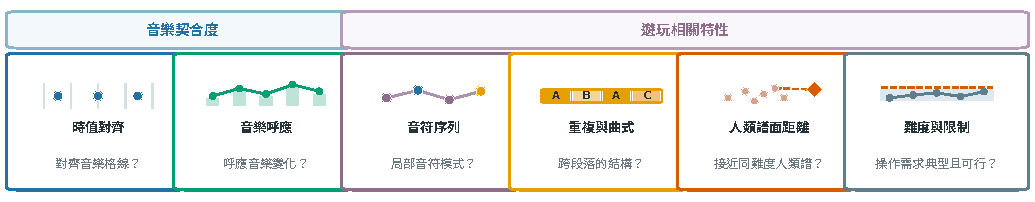
\includegraphics[width=0.96\textwidth]{figs/fig0_thesis.zh-TW.pdf}
    \refstepcounter{figure}\label{fig:overview}
    \parbox{0.94\textwidth}{\small
      \textbf{圖~\thefigure：ChartGenEval 的六個評估維度。}
      ChartGenEval 將譜面評估整理為六個彼此區分的問題，分屬音樂契合度與
      遊玩相關特性；每個維度保留各自的解讀。}
  \end{center}
}

\makeatletter
\def\@maketitle{%
  \newpage
  \null
  \vskip 2em%
  \begin{center}%
    \let\footnote\thanks
    {\LARGE \@title \par}%
    \vskip 1.5em%
    {\large
      \lineskip .5em%
      \begin{tabular}[t]{c}%
        \@author
      \end{tabular}\par}%
    \vskip .7em%
    {\large \@date}%
  \end{center}%
  \par
  \vskip .6em%
  \titlefigure
  \vskip .8em%
}
\makeatother

\sloppy
\raggedbottom

\begin{document}
\maketitle

\begin{abstract}
節奏遊戲譜面必須貼合音樂並具備良好的遊玩特性，但同一首歌曲可以容納多種
有效的音符序列。因此，與單一官方譜面的一致度會混淆有效替代方案與實際
錯誤。我們提出 ChartGenEval，一套六維度指標套件：它只使用配對官方譜面
中由作者編定的時值圖，從不以其中的音符位置作為目標。其整譜格線相位偏移
對注入的 15、30 與 60\,ms 整譜平移，中位估計都與真值一致。相較之下，
所有主要只讀譜面輸出的變化都小於人類譜標準差的 0.03 倍。

ChartGenEval 將此時值剖面與另外五個較高層次維度並列報告：音符序列、
重複與形式、音樂呼應、與同難度人類譜的距離，以及難度與可玩性限制。
各維度維持分開，不合成整體總分。九組非冗餘的擾動--測量配對，在 80 個
留出歌曲群組上皆符合預先指定的敏感度與不變性準則；32 項適用的控制檢查
亦全數通過。壓力測試也顯示，孤立代理量可能造成誤導：向常見模式改寫使語言模型
perplexity 下降 37\%，循環崩解則使自相似度上升 62\%。整體而言，這套
自動化六維度剖面可支援譜面生成模型的快速比較與迭代。各項輸出也可依角色
作為獎勵、限制或監測訊號，用於強化學習等訓練方式。
\end{abstract}

\section{引言}\label{sec:intro}

節奏遊戲的自動譜面生成把音訊映射為可遊玩的定時、定型音符序列。相關技術
已從 onset 偵測方法進展到條件式序列
模型~\cite{donahue2017ddc,halina2021taikonation,takada2023genelive,
hanzen2025tcp}。評估方法卻未同步發展。譜面規定玩家何時做什麼，因此同時
回應音樂與玩家兩端。我們以兩項要求組織評估。\emph{音樂貼合}關注音符是否
共享歌曲的時間結構，以及譜面活動是否跟隨音樂起伏；\emph{遊玩相關特性}
則包括可學習的模式、帶變化的重複，以及與指定難度相稱的要求。譜面是一項
設計作品，多種音符序列都可能滿足這些要求。

既有方法回答了有用但局部的問題。主流評估採用與單一官方譜面比較的配置
F1，量化的是重建程度：有效的替代方案會像缺陷一樣降低重合度，歌曲沒有
參照譜時也無法比較。最佳化一致度因此獎勵複製官方答案，並懲罰使製譜成為
設計問題的那些差異。語言模型（LM）似然量化模型適配度；分佈與自相似度
統計描述生成材料；玩家或專家研究則建立系統層級的體驗。這些方法各自回答
不同問題，聚合後反而會隱藏其中的權衡。

音符選擇可以自由，時值關係仍需獨立評估。傳統格線式節奏遊戲譜面以歌曲的
音樂時間框架組織音符；我們以相對外部格線的對齊來測量音樂貼合的這一部分。
配對官方譜面只提供作者編定的小節、拍號與速度圖，不以音符位置作為
目標。這項拆分保留音符選擇的自由，同時揭露只看
間隔與音符類型的統計量無法觀察的整譜平移。本文提出的格線相位偏移對注入的
15、30 與 60\,ms 平移都給出正確的中位估計，而所有主要只讀譜面測量幾乎
不變。

\textbf{ChartGenEval} 會自動計算六個維度的評估剖面：時值、音符序列、
重複與形式、音樂呼應、與同難度人類譜的距離，以及難度與可玩性。各項輸出
分為三種用途：模型改進的目標訊號、可行性限制，以及比較模型與找出問題的
監測訊號。這些用途分開處理，因此每個維度都保留自己的意義。

受控擾動提供敏感度證據。我們從人類譜出發，施加一項具有劑量控制、旨在
削弱特定性質的轉換，再檢查目標測量是否作出反應，同時要求適用的控制檢查
保持不變。九種轉換涵蓋密集時值抖動、稀疏時值錯誤、整譜平移、音符類型置換、
循環崩解、常見模式改寫、音符率縮放、爆發插入與小節順序洗牌。我們先在
40 首發展歌曲上選擇與修訂候選測量，再於 80 個留出歌曲群組上評估十組
預先指定的擾動--測量配對。所有目標與控制準則均獲滿足；其中一組配對在
代數上等價，因此留下九項非冗餘檢驗（\secref{sec:sensitivity}）。發展組
壓力測試進一步顯示，LM perplexity 可能偏好常見模式改寫，自相似度可能
偏好循環崩解，而只讀譜面測量無法察覺固定的譜面--音訊平移。

我們的貢獻如下：
\begin{enumerate}
\item \textbf{自動化的六維度回饋。} ChartGenEval 分別計算時值、音符序列、
  重複與形式、音樂呼應、人類譜距離，以及難度與可玩性的訊號。這些訊號
  可支援模型比較、快速迭代，以及以獎勵為基礎的訓練。
\item \textbf{受控擾動證據。} 九種具劑量控制的擾動，產生九項非冗餘的
  留出檢驗，檢查目標反應與指定的不變性檢查。同一設計亦揭露代理量方向反轉，
  以及只讀譜面測量對整體平移的盲點。
\item \textbf{譜面專用測量。} 套件加入格線相位偏移，以及五項處於發展階段、
  衡量譜面--音訊呼應、長程結構與同難度人類譜距離的元件。
\end{enumerate}

\section{相關研究}\label{sec:related}

\textbf{參照譜一致度。} DDC 與 Gen\'eLive! 對預測音符位置報告 F-score，
TCP 則報告 onset、onset-plus-type F1 與局部 pattern
recall~\cite{donahue2017ddc,takada2023genelive,hanzen2025tcp}。其容差與聚合
方式各異：DDC 使用 $\pm20$\,ms，Gen\'eLive! 使用 $\pm50$\,ms，TCP 則以
小節比例定義容差。TaikoNation 改以 23\,ms 二元 frame 與 pattern space
比較~\cite{halina2021taikonation}。這些都是重建估計量，承繼
\secref{sec:intro} 所述的單一參照限制。

\textbf{無配對與人類錨定評估。} DDC 以 LM perplexity 與 token accuracy
評估留出資料上的模型適配度~\cite{donahue2017ddc}。
符號音樂與文字生成研究則提供多樣性、特徵分佈、自相似度與集合層級重複
統計~\cite{li2016diversity,zhu2018texygen,yang2020evaluation,dong2020muspy,
wu2020jazz}。人類研究回答另一個問題：MuTE 以專家評分驗證參照對齊的鋼琴
編曲測量~\cite{gover2022mute}；Gen\'eLive! 報告專業部署
回饋~\cite{takada2023genelive}；Mania Archetype 則結合參照相似度與八位
資深玩家評分~\cite{wang2024mania}。ChartGenEval 提供這類人類研究可進一步
採用的自動測量與擾動敏感度證據。

\textbf{指標壓力測試與時值。} SCHmUBERT 建構非音樂性的 piano roll，卻能
匹配逐 frame 自相似統計~\cite{plasser2023schmubert}。Fr\'echet Music
Distance 以音高與力度擾動測試，但仍是集合層級的 embedding
距離~\cite{retkowski2025fmd}。STRUM 在逐歌搜尋整體偏移後報告參照 onset
F1~\cite{opria2026strum}；ChartGenEval 則把整譜格線相位偏移作為譜面層級
測量，且不以參照音符作為目標。我們的 6\,ms 時值容差以時間辨別研究為
依據~\cite{friberg1995jnd,london2012hearing}（\secref{sec:timingmethod}）。

\section{方法}\label{sec:methods}

\subsection{ChartGenEval 指標套件}\label{sec:suite}

ChartGenEval 自動計算六組測量。受控擾動檢查目標測量在不同劑量下的敏感度，
適用的控制檢查則確認不變性。
\tabref{tab:suite} 區分本文提出的測量與既有譜面統計量的改編版本，並列出
每一角色在本研究中獲得的最強證據。

\begin{table*}[t]
\centering
\footnotesize
\setlength{\tabcolsep}{5pt}
\renewcommand{\arraystretch}{1.15}
\begin{tabular}{@{}p{0.135\textwidth}p{0.375\textwidth}p{0.165\textwidth}p{0.235\textwidth}@{}}
\toprule
構念 & 主要輸出與解讀 & 來源 & 證據基礎 \\
\midrule
時值 & 格線容差內比例與殘差尾部；整譜格線相位偏移 &
本文提出的譜面對格線剖面 & 使用作者編定格線的 C1、C1s、C2 留出檢驗 \\
音符序列 & LM loss 作為描述；未見轉移懲罰作為單側熟悉度檢查 &
改編的 $n$-gram 統計 & C3 留出檢驗（轉移熟悉度） \\
重複與形式 & 4-gram 典型性；ABAB 交互回應；停滯--疏離代理量 &
改編的 4-gram 分數；兩項本文提出的測量 &
C4、C5、C8 留出檢驗（單一 4-gram 軸）；新測量僅有發展組證據 \\
音樂呼應 & 小節層級密度--能量等級相關；連打首音 onset 支持度 &
兩項本文提出的測量 & 僅有發展組證據 \\
人類譜距離 & 32 維譜面表徵中，到 20 張最近訓練譜的平均距離 &
本文提出的譜面專用實例 & 僅有發展組證據 \\
難度與限制 & 密度與負荷典型性；過載與密度尖峰限制 &
改編統計量；本文提出的校準 & C6、C7 留出檢驗（密度典型性、尖峰限制） \\
\bottomrule
\end{tabular}
\caption{ChartGenEval 的構念、來源與證據邊界。各構念所需的時值、音訊、
格線或參照錨點，見方法一節（\secref{sec:data}、\secref{sec:layers}）。
「本文提出」表示測量由本文定義，其中的基礎統計量可能已有既有來源。
留出證據只適用於表中具名輸出。}
\label{tab:suite}
\end{table*}

ChartGenEval 的所有輸出都可自動計算，但用途不同。具有明確方向的輸出可
作為獎勵或懲罰，可玩性檢查可作為限制，描述性輸出則可作為監測訊號。
強化學習等訓練方式可依任務選擇這些訊號並設定權重。

本文提出的測量針對單一譜面統計量留下的缺口設計。\emph{整譜格線相位偏移}
在固定的小節、拍與八分音符錨點上搜尋 $-250$ 至 $+250$\,ms 的平移量。
為檢查活動是否跟隨音樂起伏，\emph{密度--能量呼應}在作者編定的小節視窗內，
計算每秒打擊數與線性 mel 能量的 Spearman 相關。可用視窗少於八個，或歌曲
能量的第 90 與第 10 百分位差小於其中位數的 5\% 時，這項測量記為不可用。
\emph{連打首音 onset 支持度}是節奏群群首中，在三個 mel frames
（約 $\pm35$\,ms）內的最大 spectral flux 達到該歌曲第 60 百分位門檻者
所占比例。相鄰 onset 的間隔至少為 0.25\,s 時才開始新群組，以免密集連打
主導分母。

對長程結構而言，\emph{交互回應}把譜面依十六分音符位置切成兩小節樂句。
具一個位置容差、經機率校正的節奏相似度，乘上經機率校正的音色一致度。
若 $S(i,j)$ 表示這個乘積，分數就是 $S(i,i+2)[1-S(i,i+1)]$ 的樂句平均：
素材隔著中間樂句回返，但相鄰的複製式重複不會得到獎勵。

\emph{停滯--疏離代理量}使用活動小節的節奏與音色 fingerprints。若某小節是
連續相似度 $\geq.8$ 序列中的第四個或之後成員，或其每個可用的 16 音符
音色視窗都呈現週期不超過四的精確循環，便標為停滯。若前後 32 小節內都
沒有相似度至少 .75 的小節，便標為疏離。原始輸出是兩類集合聯集占所有
活動小節的比例。我們只把它作為結構訊號。最後，\emph{人類譜距離}以
32 個音符間隔、音符類型、密度與多樣性
特徵表示每張譜。特徵依難度標準化，原始距離 $g$ 是到同難度 20 張最近
訓練譜的平均歐氏距離。有界的顯示分數為 $\exp(-g/a)$，其中 $a$ 是該
course leave-one-out 距離的第 90 百分位。表徵本身為譜面專用，其中的
entropy、bigram 與最近鄰基礎量則是既有統計方法。

\subsection{資料與時值參照}\label{sec:data}

我們使用自網路社群資源蒐集的 taiko 風格譜面檔與對應音訊；譜面檔轉錄
官方難度 course，並作為人類參照譜。由於譜面與音訊可能受版權保護，語料
本身不隨本文發布。來源紀錄依歌曲合併為群組，不一致的來源對映予以排除。
訓練集與測試集各有不同用途。訓練集有 924 筆來源紀錄，涵蓋 813 個不重複
的歌曲群組與 3{,}880 張各難度譜面；這些譜用於擬合校準值與 LM。測試集有
140 筆來源紀錄，形成 120 個歌曲群組。前 40 組含 170 張人類譜，作為指標
與擾動設計、圖表及系統剖面的發展組；後 80 組含 333 張各難度譜面，作為
確認性檢驗的留出組。資料另含 80 個歌曲群組的驗證集；本文報告的分析未使用。
發展與留出兩階段的受控擾動分析合計涵蓋全部 120 首測試歌曲：40 首用於
發展，80 首用於留出確認。公開系統比較只使用其中 40 首發展歌曲。

另五項本文提出的元件是在發展組上選擇與修訂，因此相關證據仍屬探索性。
附錄~\ref{app:protocol} 記錄資料組建構方式與完整分析規格。

時值需要外部的歌曲時值參照。主要格線使用配對官方譜面檔中，由作者編定的
逐小節時間戳、拍號與速度中繼資料；官方譜面的音符時間與類型從不作為目標。
換言之，官方檔案提供的是時值圖，不是唯一正確的音符序列。這保留時值圖中
精確的小節結構，也讓生成譜能在同一音樂時間框架內採取不同而有效的音符
設計。我們不使用生成譜自行宣告的格線，避免讓生成器定義自己的參照。

作者編定時值圖不可得時，我們另以音訊估計 downbeat 作為發展階段的替代
方案。40 首發展歌曲中，有 39 首的估計節拍週期與中繼資料週期相差不超過
2\%；其餘一首相差 2.39\%。絕對偏移使用作者編定格線報告，其小節相位
直接來自時值圖。只有具作者編定時值圖的 course 才納入留出時值分析；其餘
course 的時值測量記為不可用。

\subsection{測量角色與難度校準}\label{sec:layers}

每張譜都是定時、定型的音符序列。我們依 \figref{fig:overview} 的六個問題
組織原始測量，並對應 \secref{sec:intro} 的兩項要求。音樂貼合關注所聽與
所打的一致，因此時值與音樂呼應需要歌曲；其餘四組不需音訊，用來描述遊玩
特性，其中本文提出的結構測量另需節拍格線。改編的譜面內部基礎量包括
平滑化 trigram LM、未見轉移率、音符率、局部密度、短間隔負荷、entropy，
以及獨特或重複的 4-grams。我們保留 trigram 負對數似然（NLL）作為 LM
適配度描述；perplexity 是其指數。我們另把 NLL 轉換為依難度條件化的範圍
分數，稱為\emph{pattern-IC 典型性}。未見轉移率則提供單側的\emph{轉移
熟悉度}檢查：訓練語料中未見的 trigram，代表對語料而言不熟悉，不代表
語義上無效。本文提出的結構、音訊呼應、時值與人類譜距離測量已在
\secref{sec:suite} 定義。

我們把選定特徵轉成\emph{同難度範圍分數}。對每個 course 與選定特徵，
令 $l,u$ 分別為訓練譜的第 10、90 百分位，
$h=\max((u-l)/2,10^{-9})$ 為受保護的半範圍寬。兩側使用同一尺度：
\begin{equation}
\begin{aligned}
d(x)&=
\begin{cases}
(l-x)/h, & x<l,\\
0,       & l\leq x\leq u,\\
(x-u)/h, & x>u,
\end{cases}\\
s(x)&=\frac{1}{1+d(x)^2}.
\end{aligned}
\label{eq:band}
\end{equation}
因此範圍內得 1，向下與向上等距偏離得到相同分數。我們同時保留帶號距離，
使大幅偏離不會塌縮到同一個近零分數。

這個分數衡量譜面對指定難度而言有多不尋常；它本身不判定譜面品質。有些
測量具有明確的不可欲方向，例如超出難度相對限制的過度負荷；它們使用另行
具名的單側分數。轉移熟悉度相對訓練語料同樣是單側的，但不意味語義上
無效。沒有指定校準的同族測量保留為原始描述。entropy、密度與重複都沒有
通用方向：每一項都可能過低或過高。受控擾動顯示，目標變化往往會把這些值
推出人類範圍；不尋常但仍可玩且貼合音樂的譜面，仍可能反映創意選擇
（\secref{sec:discussion}）。

可玩性限制維持為分開且不可補償的可行性檢查。發展組的人類譜中，音符率、
短間隔與密度尖峰檢查分別有
88\%、89\% 與 97\% 得分至少 0.99。整體平移估計等數值則維持描述性。

\subsection{對歌曲測量時值}\label{sec:timingmethod}

我們把低於 6\,ms 的格線偏差視為容差內，其尺度取自已發表的短間隔恰可
覺差~\cite{friberg1995jnd}。更大的誤差分三個範圍報告：超過 6、12、18\,ms。
相鄰音符間隔另以
$\max(6\,\mathrm{ms},2.5\%\times\mathrm{IOI})$ 的容差比較。每個音符
被計為容差內、超過三個範圍之一，或未配對。未配對的生成音符留在分母中，
因此新增離格音符會降低容差內比例。此量沒有參照音符 recall 項，因此刪除
未配對的生成音符可能提高比例；我們把它與音符數和同難度密度一併解讀。
分析先對每張譜摘要，再跨譜報告中位數與尾部。

共同平移 $\delta$ 不會改變任何相鄰音符間隔：
\begin{equation}
(t_{i+1}+\delta)-(t_i+\delta)=t_{i+1}-t_i.
\label{eq:shift-invariance}
\end{equation}
音符類型也不變，因此以這些間隔與類型為基礎的只讀譜面測量不變或幾乎不變。

最近格點配對可能錯過恆定平移（\figref{fig:timing}）。在密格線上，每個被
平移的音符可能只是與另一個鄰近格點配對，因此我們改對整張譜估計單一偏移。
令 $G_k$ 表示固定的小節、拍與八分音符格線，並定義
$d(x,G_k)=\min_{g\in G_k}|x-g|$。對音符時間 $t_i$，候選平移的分數為
\begin{equation}
\begin{aligned}
S(\delta)
 &= \sum_k w_k\,\frac{1}{n}\sum_i
 \left[1-\frac{d(t_i-\delta,G_k)}{\tau}\right]_+,\\
\hat{\delta}
 &= \operatorname*{arg\,max}_{\delta\in[-250,250]\,\mathrm{ms}}
 S(\delta),
\end{aligned}
\label{eq:phase-offset}
\end{equation}
其中 $[z]_+=\max(z,0)$、$\tau=12$\,ms，小節、拍與八分音符格線的權重
依序為 0.2、0.3 與 0.5。搜尋間隔為 0.5\,ms。作者編定格線來自官方譜面的
時值圖，而非其音符序列；音訊估計格線則由音訊 downbeat 推估。合併三種
格線可消解多數週期性平手；近似平手時，取幅度最小的偏移。
兩種時值摘要都必須有上述其中一種外部格線；作者編定時值圖與音訊估計格線
皆不可得時，時值結果記為不可用。BPM 只提供週期、不提供相位，因此不足以
作為時值參照。

\begin{figure*}[t]
\centering
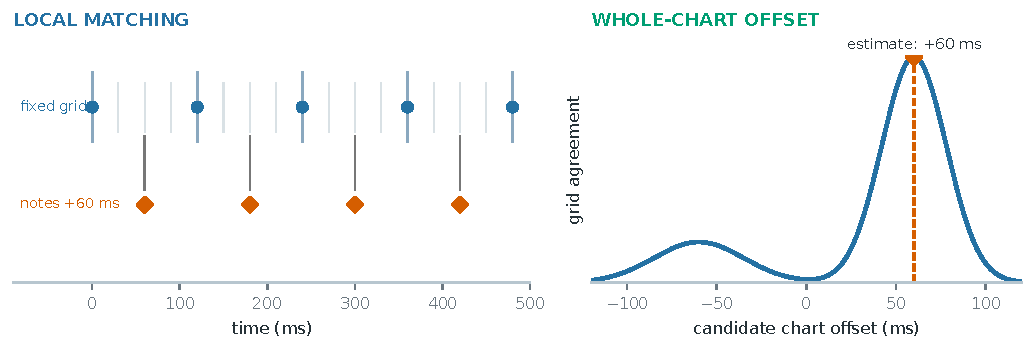
\includegraphics[width=0.94\textwidth]{figs/figT_timing_alignment.pdf}
\caption{為何時值需要整譜估計。\textbf{左}：最近格點配對可能把平移後的
音符配到不同細分點，因而報出很小的局部誤差。\textbf{右}：我們測試候選的
整譜偏移；圖中的示意一致性曲線最高點位於注入的 $+60$\,ms 平移。
格線在評估生成譜面之前即已固定。}
\label{fig:timing}
\end{figure*}

\subsection{受控擾動與判定準則}
\label{sec:probes}

\begin{table*}[t]
\centering
\footnotesize
\setlength{\tabcolsep}{4pt}
\begin{tabular}{@{}p{0.30\textwidth}p{0.18\textwidth}p{0.46\textwidth}@{}}
\toprule
受控擾動（強度） & 改變的性質 & 預先指定的反應 \\
\midrule
C1 時值抖動（$\pm$10/20/30\,ms） & 音符時值 &
時值容差內比例 $\downarrow$ \\
C1s 稀疏時值錯誤（名目 0.5/1/2\%，$\pm$60\,ms） & 少數音符時間 &
絕對時值誤差 p99 $\uparrow$ \\
C2 整體平移（+15/30/60\,ms） & 譜面--音訊對齊 &
絕對格線相位偏移 $\uparrow$ \\
C3 音符類型置換（$p{=}0.2/0.4/0.8$） & 局部轉移 &
轉移熟悉度 $\downarrow$ \\
C4 循環崩解（$p{=}0.3/0.6/1$） & 重複與形式 &
4-gram 典型性 $\downarrow$ \\
C5 常見模式改寫（$p{=}0.3/0.6/1$） & 模式多樣性 &
4-gram 典型性 $\downarrow$（單一有效軸） \\
C6 音符率縮放（$\times$0.5/1.5/2） & 難度適配 &
音符率典型性 $\downarrow$ \\
C7 爆發插入（2/4/8 個叢集） & 局部過載 &
密度尖峰限制 $\downarrow$ \\
C8 小節順序洗牌（$p{=}0.3/0.6/1$） & 全局形式 &
4-gram 典型性 $\downarrow$ \\
\bottomrule
\end{tabular}
\caption{受控擾動及其九項非冗餘目標讀數。C3--C5 保留音符時間，C4 與
C6 則保留或控制密度。C5 原先具名的兩個 4-gram 輸出在代數上等價，因此
只計為一個有效軸。pattern-IC 典型性與原始 trigram NLL 保留為不預設方向
的次要分析。附錄~\ref{app:corruptions} 提供視覺化前後比較與完整轉換規格。}
\label{tab:probes}
\end{table*}

發展組反應矩陣屬描述性分析。它報告最大劑量的標準化變化，以及逐譜淨方向：
相對各自原譜上升的譜面比例減去下降比例。完整的發展組計算與 C5 的獨立 LM
檢查見附錄~\ref{app:protocol}。

我們在 80 個留出歌曲群組上評估十列預先指定的擾動--測量配對。五個確定性
擾動複本先在每張譜、每個劑量內平均，各 course 再於歌曲內平均，因此歌曲
是推論單位。每項檢驗使用定向後的劑量相關，以及最大劑量減 sham 對比。
我們計算歌曲群組 bootstrap 區間，並對十列套用 Bonferroni 校正的 99.5\%
區間。若至少 72 首歌曲可評、所有必要控制均通過，且兩個調整後
上界皆低於零，該反應即符合準則。完整協定見附錄~\ref{app:protocol}。

各項控制與對應測量家族所主張的不變性一致，包括精確重算、音符與格線共同
平移、時值與密度測量使用的 Don--Ka 音色雙射，以及只讀譜面測量使用的
整譜平移。必要控制若未通過，該目標反應便不能計為受到支持。

\subsection{受評系統}\label{sec:systems}

我們評估五個公開生成器，涵蓋三種音符格式：太鼓音符類型、僅含時值的
onset 串流，以及 osu! 位置型物件。兩個系統產生太鼓音符類型：
Mapperatorinator v32~\cite{mapperatorinator} 是社群開發、採 MIT 授權的
多模式 osu! beatmap 生成框架，本研究以 taiko 模式評估；另一個是 FDG
發表的 TaikoNation~\cite{halina2021taikonation}，本研究直接執行作者公開的
研究 repository。另外三個系統只進入時值與音樂呼應測量：Dance Dance
Convolution 的 onset 管線（ddconset）~\cite{donahue2017ddc}、Gen\'eLive!
的公開 timing-only 配置~\cite{takada2023genelive}，以及以 osu! 難度為
目標的生成器 AutoOsu~\cite{autoosu}。全部系統都在其公開推論配置下，從
音訊為同一批 40 首發展歌曲製譜。本研究未在此語料上訓練或微調這些系統，
但這些商業歌曲與各系統訓練資料的重疊無法排除
（\secref{sec:limitations}）。course 對映如下：
Mapperatorinator 使用相應的太鼓 course；Gen\'eLive 的 Beginner、Easy、
Medium、Hard、Challenge 設定分別對映到 Easy、Normal、Hard、Oni、Ura，
歌曲無 Ura 譜時，Challenge 以 Oni 為參照 course；單一設定系統則使用
指定的 Oni 參照。同一音符格式共用轉換至評估事件串流的程序
（\secref{sec:systemresults}）。同批歌曲的人類譜提供參照列。依難度生成的
系統對每個可得 course 各產生一張譜（170 或 200 張）；其餘系統每首歌
產生一張（40 張）。我們將這些剖面報告為描述性的發展組分析。

\section{結果}\label{sec:results}

\subsection{九項有效檢驗符合留出準則}
\label{sec:sensitivity}

十列預先指定的配對皆符合兩項反應準則，32 項適用的控制檢查全數通過，而且
每項分析都保留 80 個歌曲群組（\tabref{tab:confirmation}）。兩列 C5 在
代數上等價，因此結果代表橫跨七個有效輸出軸的九組非冗餘擾動--測量配對。

\begin{table*}[t]
\centering
\scriptsize
\setlength{\tabcolsep}{3.5pt}
\begin{tabular}{@{}llrll@{}}
\toprule
配對 & 主要反應 & Courses & $\bar\rho_{\mathrm{dose}}$ [99.5\% CI] &
$\overline{\Delta}_{\mathrm{max-sham}}$ [99.5\% CI] \\
\midrule
C1  & 時值容差內比例 & 333 & $-.744\;[-.815,-.667]$ & $-.502\;[-.558,-.446]$ \\
C1s & 絕對時值誤差 p99 & 332 & $-.234\;[-.344,-.134]$ & $-.306\;[-.508,-.144]$\,ms \\
C2  & 絕對格線相位偏移 & 333 & $-.916\;[-.981,-.826]$ & $-55.58\;[-61.43,-49.83]$\,ms \\
C3  & 轉移熟悉度 & 333 & $-.800\;[-.856,-.737]$ & $-.231\;[-.262,-.199]$ \\
C4  & 4-gram 典型性 & 333 & $-.445\;[-.573,-.312]$ & $-.165\;[-.226,-.108]$ \\
C5  & 4-gram 典型性 & 333 & $-.358\;[-.459,-.258]$ & $-.131\;[-.189,-.078]$ \\
C6  & 音符率典型性 & 333 & $-.693\;[-.784,-.579]$ & $-.582\;[-.672,-.483]$ \\
C7  & 密度尖峰限制 & 333 & $-.940\;[-.950,-.930]$ & $-.619\;[-.644,-.593]$ \\
C8  & 4-gram 典型性 & 330 & $-.589\;[-.728,-.435]$ & $-.224\;[-.293,-.156]$ \\
\bottomrule
\end{tabular}
\caption{80 個歌曲群組上的留出結果。定向後數值越大
越好，因此目標敏感度表現為負的劑量相關，以及負的最大劑量減 sham 對比。
九組有效配對皆符合預先指定的準則；區間為家族校正的 99.5\% 歌曲群組
bootstrap 區間。C5 報告兩列代數等價輸出中的一列。}
\label{tab:confirmation}
\end{table*}

32 項控制皆精確維持不變。C1s 保留 332 個完整 course，C8 保留 330 個，
其餘配對各保留 333 個。樣本數與排除原因見附錄~\ref{app:protocol}。

\paragraph{C5 只提供一個有效軸。}\label{sec:dependency}
重複 4-gram rate 正好等於一減 unique 4-gram rate，因此兩者的鏡像對稱
範圍分數，除浮點捨入誤差外完全相同。預先指定的兩個 C5 輸出名稱不能視為
彼此獨立的佐證；C5 支持的是單一有效 4-gram 重複／唯一性反應。

\subsection{外部時間可偵測譜面--音訊平移}
\label{sec:anchorresults}

一張譜的密度、模式與音符類型可以看似合理，同時相對音樂偏晚。C2 將每個
音符平移 15、30 或 60\,ms。在發展組上，沒有任何主要只讀譜面輸出的變化
超過人類標準差的 0.03 倍，因為只看間隔與類型的測量對共同平移保持不變。

最近格點配對也會錯過平移：密格線可能把每個被平移的音符配到另一個鄰近
細分點。兩種參照來源的格線相位偏移搜尋，都回傳 15.00、30.00 與
60.00\,ms 的中位估計。每個來源、每個平移量下，至少 169/170 張譜落在
注入值的 3\,ms 內。連打首音 onset 支持度也會在音符 onset 處作出反應
（各強度淨方向 $-0.74$ 至 $-0.88$），並在音符時間保留時保持不變。
密集時值抖動下，每張譜在每個強度的 6\,ms 內音符比例都下降；在
$\pm10$\,ms 時，容差外比例的實測中位數為 0.40，符合
$P(|U(-10,10)|>6)=0.4$。

稀疏錯誤需要尾部敏感的讀數。在 C1s 下，最近格點會重新配對多數被移動
音符，因此平均時值誤差的跨譜中位數維持為零。時值誤差 p99 在留出檢驗中
作出反應；音符序列 LM 也會改變，因為移動一個音符會改變兩個相鄰間隔。
密度實質不變，形式則只有微弱反應。

\subsection{目標擾動揭露代理量的有利移動}
\label{sec:reductio}

\begin{figure*}[t]
\centering
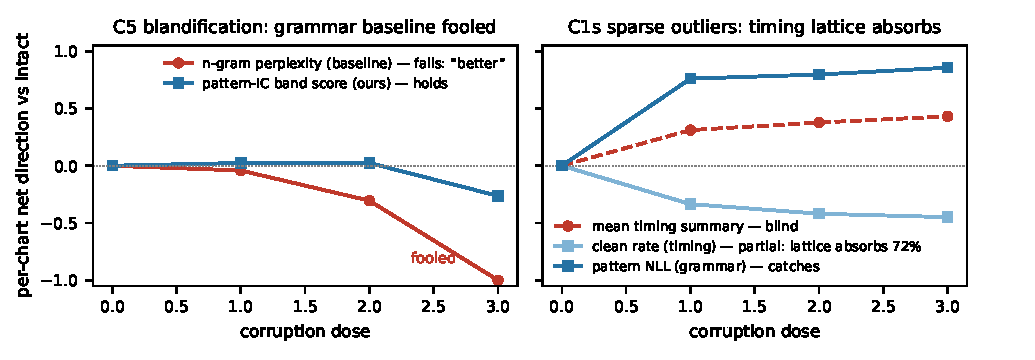
\includegraphics[width=0.92\textwidth]{figs/figA_complementarity.pdf}
\caption{一項測量錯過目標變化、另一項測量作出反應的兩個案例。長條顯示
相對原譜上升的譜面比例減去下降比例；由淺至深表示發展組上的三個擾動強度
（僅為描述性結果，不是把各譜視為獨立樣本的信賴敘述）。\textbf{左}：
常見模式改寫使 LM loss 下降、pattern-IC 範圍分數上升，4-gram
重複／唯一性軸則往反方向移動（兩個代數等價的輸出名稱只繪一次）。
\textbf{右}：稀疏的 $\pm60$\,ms 時值錯誤使平均時值誤差接近零，且多被
最近格點重新配對；音符序列 LM 則回應改變後的間隔。}
\label{fig:complementarity}
\end{figure*}

兩個借用的指標，在目標擾動下朝名目上較有利的方向移動
（\figref{fig:complementarity} 左）。\emph{Perplexity 偏好常見模式}：
發展組人類譜的平均值為 9.44；向 LM 最常見模式改寫後，perplexity 下降
37\%（9.44 $\to$ 5.98）。Dance Dance Convolution 把 perplexity 作為留出
人類譜上的模型適配度~\cite{donahue2017ddc}；若將它移植為生成結果的無參照
品質讀數，「越低越好」的解讀便會偏好改寫後的譜面。這是似然／品質背離
在譜面層級的實例~\cite{theis2016note}。一個 LM 產生改寫、另一個 LM
評分時，反轉仍然存在（9.44 $\to$ 6.04，$-36\%$）。pattern-IC 範圍分數
隨三個劑量上升並移向人類範圍。在留出次要分析中，其最大劑量變化為
$+0.021$，nominal 95\% 區間為 $[-0.034,0.077]$；原始 trigram NLL 則從
2.087 降至 1.715（$-0.373$，$[-0.399,-0.346]$）。因此，典型性本身無法
修正此案例。有效 4-gram 軸（\secref{sec:dependency}）在發展組上從
0.99 降至 0.87。

\emph{自相似度偏好崩解}：以譜面自身最主要的 4-gram 循環取代原譜，使
自相似結構度~\cite{wu2020jazz}上升 62\%（0.0848 $\to$ 0.1370），集合層級
Self-BLEU~\cite{zhu2018texygen}則從 0.845 上升至 0.898。複製貼上的輸出
依構造會更加自相似，但 4-gram 重複／唯一性分數從 0.99 降至 0.83。

另外兩項觀察結果補足論證。\emph{方向不穩定}：對
\secref{sec:systemresults} 兩個公開可得、輸出位於人類語料高 entropy 側的
太鼓生成器，perplexity 以預期方向區分人類與生成譜（AUC 0.80）；但 C5
顯示相同讀法在低 entropy 側會反轉。若帶號品質指標的方向取決於系統位在
人類分佈的哪一側，它便無法支持穩定排名；同難度範圍分數把兩側一致解讀為
偏離典型性。C5 顯示該分數為何必須與 4-gram 重複／唯一性軸一併閱讀。
\emph{譜長混淆}：在相同系統池上，type--token ratio 與音符數的相關為
$|\rho|=0.85$，distinct-2 為 $0.56$，範圍分數則至多為 $0.28$。

這些案例確立了互補性，卻沒有提供聚合權重。因此，我們讓各輸出維持分開，
不以單一總分隱藏其中的權衡。完整的指標--擾動反應矩陣見附錄中的
\figref{fig:responsemap}。

\subsection{本文所提元件的發展組證據}
\label{sec:newmetricresults}

\tabref{tab:suite} 中另五項元件具有描述性的發展組證據。把原譜與三個劑量
合併計算的 Spearman 反應，支持彼此不同的操作角色。交互回應在循環崩解與
小節洗牌下下降（$\rho=-.612$ 與 $-.506$），在時值抖動與整體平移下則
幾乎不變（$-.086$ 與 $-.003$）。停滯--疏離代理量對循環崩解有強烈反應
（定向為越大越好後 $\rho=-.924$），在時值抖動與整體平移下變化很小
（$-.007$ 與 $+.010$）。這些結果支持對目標結構變化的敏感度。

兩項音訊呼應測量捕捉不同時間尺度。連打首音 onset 支持度在整體平移下
下降（$\rho=-.559$）；小節層級密度--能量呼應在一致密度縮放下保持穩定
（$\rho=+.005$），在小節洗牌下下降（$\rho=-.386$）。它對爆發插入的反應
偏弱（$\rho=-.092$），因此其解讀限於小節尺度共變。依難度計算的人類譜
差距描述的是聯合特徵分佈：它能標示不同於訓練點雲的特徵組合，卻不把
不尋常譜面分類為創意或品質不佳。在 C3--C8 下，其同難度分數的最大劑量
淨方向介於 $-.32$ 與 $-.88$；整體平移下的中位變化為零。

\subsection{系統剖面}
\label{sec:systemresults}

\figref{fig:tiers} 與 \figref{fig:profiles} 的描述性系統剖面分開呈現兩種
會被單一數字合併的效果：相近的時值摘要比例可能源自不同時值行為，而指定
course 也可能改變只讀譜面測量的解讀。

\begin{figure*}[t]
\centering
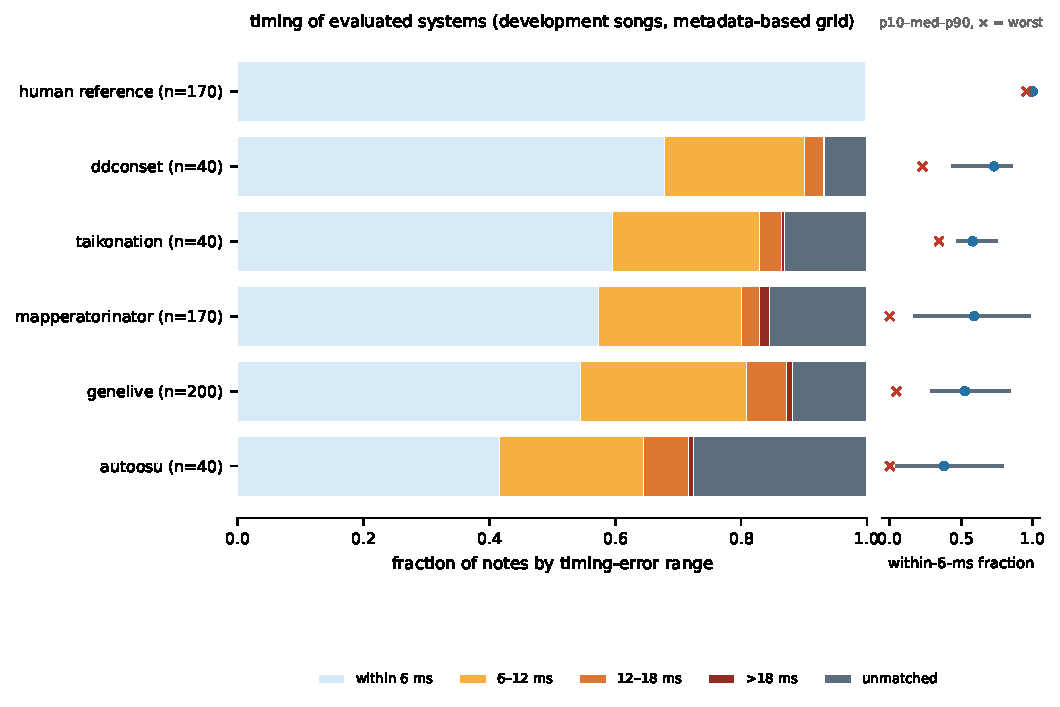
\includegraphics[width=0.92\textwidth]{figs/figB_timing_tiers.pdf}
\caption{受評系統在 40 首發展歌曲上的時值，使用作者編定格線。每條顯示
落在 6\,ms 內、6--12、12--18、18\,ms 以上或未配對的平均音符比例；$n$
為譜面數。右側橫線涵蓋 6\,ms 內比例的第 10--90 百分位，圓點標示中位數，
倒三角形標示最小值。相近的平均容差內比例，仍可能伴隨不同的時值尾部。}
\label{fig:tiers}
\end{figure*}

\begin{figure*}[t]
\centering
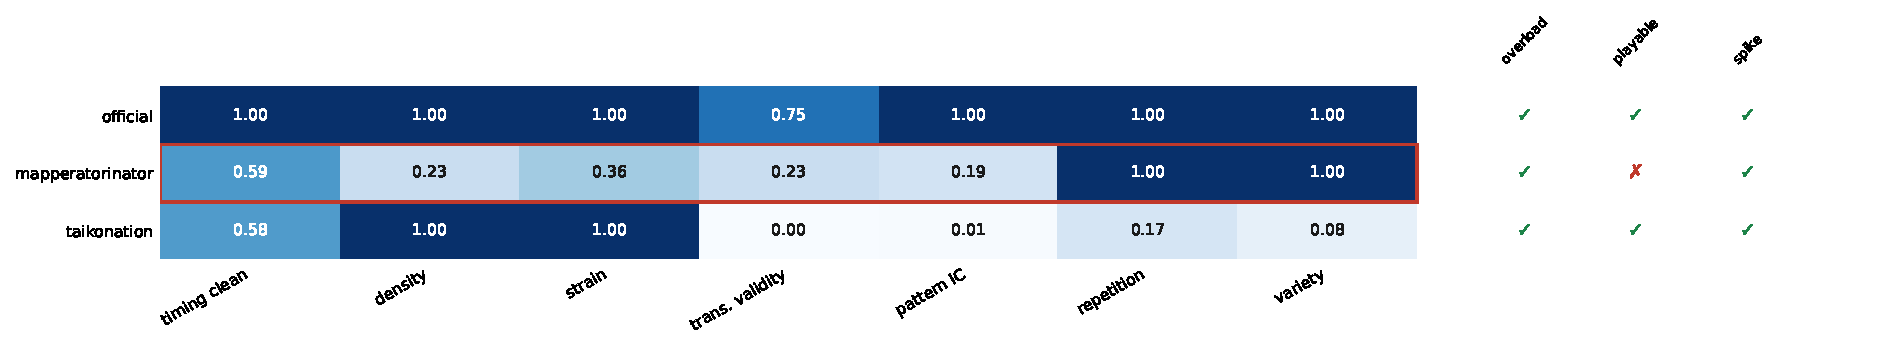
\includegraphics[width=0.92\textwidth]{figs/figD_profile_matrix.pdf}
\caption{人類參照與兩個使用太鼓音符類型的生成器，在發展組上的分開結果。
第一欄是音符落在格線 6\,ms 內的中位比例；其餘格為 $[0,1]$ 的校準分數。
音符率、短間隔、局部模式與 4-gram 重複／唯一性各欄的 1 表示中位數落在
人類範圍；轉移熟悉度是單側分數（越大越好），連人類參照也只有 0.75，
因為 LM 仍會遇到未見的 trigrams。右側符號以中位閾值 0.5 分開顯示過載、
尖峰與可玩性檢查。其他音符格式只出現在時值比較
（\figref{fig:tiers}）。各欄揭露不同偏離，不合成總分。}
\label{fig:profiles}
\end{figure*}

\textbf{相似的時值比例可能源自不同原因。} 在\figref{fig:tiers}中，近乎
為一的人類列是以作者編定小節 metadata 作為參照的一致性檢查，不是模型
結果。兩個太鼓系統落在 6\,ms 內的音符中位比例幾乎相同（0.59 與 0.58），
其餘時值行為卻不同：Mapperatorinator 有 10\% 的相鄰間隔超出相對容差，
TaikoNation 則為 41\%。格線相位偏移搜尋得到 26 與 55\,ms 的中位偏移；
最近格點配對對兩者卻都報告不到 1\,ms 的 6\,ms 容差外平均誤差。
TaikoNation 的譜面活動與音訊能量也幾乎無關（相關 $-0.003$），音符落在
平均能量的 frame 上。DDC onset 系統在相同音訊上得到 2.5\,ms 偏移，可作為
共享解碼偏移的控制。與 Mapperatorinator 共用 osu! 轉換路徑的 AutoOsu
讀出 19\,ms 中位偏移；不同數值排除了共同轉換常數作為唯一解釋
（\secref{sec:systems}）。

\textbf{指定 course 會改變讀數。} Mapperatorinator 的生成／人類音符率比
從 Easy、Normal 的 2.15--2.35，降至 Oni 的 1.31 與 Ura 的 1.07
（附錄中的\figref{fig:difficulty}）。其音符率、短間隔與局部模式分數在
Easy 至 Hard 低於 0.5，在 Oni 與 Ura 則接近 1。時值沒有相同趨勢：
落在 6\,ms 內的中位比例依序為 0.56、0.60、0.59、0.57 與 0.62。因此，
證據支持的是難度不匹配，不是高難度下的全面改善。TaikoNation 只有單一
設定；在該設定下，音符率與短間隔負荷落在人類範圍，卻有 55\% 的 trigrams
未見於依難度訓練的 LM，重複 4-gram rate 為 0.004。

\section{討論}\label{sec:discussion}

ChartGenEval 為譜面生成器提供可自動計算的六維度回饋。留出檢驗顯示，
七個有效輸出軸會回應各自的目標變化；發展組分析也找出常用代理量的盲點。
這套剖面可用來比較模型版本，並指出變化發生在哪一個維度。具有明確方向的
輸出可作為獎勵或懲罰，可玩性檢查可作為限制，描述性輸出則可作為監測訊號。
強化學習可依任務選擇這些訊號並設定權重。

\textbf{非典型性必須結合脈絡解讀。} 受控擾動顯示，目標變化往往會把分數
推出同難度人類範圍，但反向推論並不成立：不尋常譜面可能反映創意選擇。
時值與可行性檢查有助於解讀這項偏離。當訊號不一致時，剖面會直接呈現
其中的權衡。
距離尺度可協助理解大幅偏離：發展組人類譜在序列軸上的最大值為 4.8 個
半範圍寬，Mapperatorinator 與 TaikoNation 的中位數則分別為 2.1 與 12。

\textbf{可轉移性取決於測量角色。} 時值與音樂呼應測量只讀音符時間，因此
可直接施用於三種音符格式。序列、形式與距離測量需要目標遊戲的 tokenizer，
以及供校準的人類譜；lane、位置或方向 token 都可取代太鼓音符類型。相同的
受控擾動設計可檢查哪些反應能轉移到另一款遊戲。位置型遊戲還需要移動成本、
手部分配與旋轉等額外檢查。

\section{限制}\label{sec:limitations}

\textbf{證據範圍。} 受控擾動顯示測量會對已知變化作出反應；它們不直接
測量玩家體驗。九種擾動未涵蓋配錯歌曲、刪除音樂上
重要的音符，以及刻意離格配置。個別譜面在擾動後也可能移向人類範圍。
另五項元件只有發展組證據。最後，預先
指定的兩個 C5 輸出名稱在代數上等價；未來研究應改測獨立的結構測量。

\textbf{語料與系統範圍。} 人類範圍由單一遊戲語料定義，其難度與速度涵蓋
彙整於附錄~\figref{fig:coverage}。其他音符格式只接受時值與音樂呼應測量，
每個公開系統也只以一個公開配置與一個 seed 執行。發展歌曲與系統訓練語料
可能重疊，本研究未加以控制。
共用路徑比較顯示，單一轉換常數不足以解釋觀察到的所有偏移，但各格式特定
的轉換效應仍可能存在。因此，系統結果屬比較性描述。

\textbf{測量與推論。} 時值容差內比例會懲罰新增的離格音符，卻沒有參照
recall 項，因此刪除音符可能提高比例；這項測量也需要外部格線。留出時值
結果使用作者編定格線，音訊估計替代方案則只有發展組證據。序列 token 包含
音符間隔，因此時值與序列反應可能重疊（附錄中的\figref{fig:responsemap}）。
各 course 先在歌曲內平均，因此歌曲是推論單位。確定性的擾動複本在譜內
平均，不會形成額外樣本。

\FloatBarrier

\section{結論}\label{sec:conclusion}

我們提出 ChartGenEval，一套六維度指標套件。它以配對官方譜面作為作者
編定的時值圖，同時排除其中的音符位置，不把它們當成目標。時值與另外五個
較高層次維度並列報告；原始描述、雙側典型性與單側可行性檢查保留各自
角色，不合成整體分數。

九組非冗餘擾動--測量配對，在 80 個歌曲群組上皆符合留出敏感度與不變性
準則。同一研究顯示，只讀譜面測量會錯過整體平移，perplexity 與自相似度
則可能在目標擾動下朝名目上有利的方向移動。

這套剖面提供自動化回饋，可用來比較與迭代譜面生成器。具有明確方向的輸出
可引導以獎勵為基礎的最佳化，可行性檢查可作為限制，描述性輸出則可追蹤
模型行為。這種依角色使用訊號的設計可支援強化學習，同時讓各維度維持分開。

\section*{倫理聲明}
本研究使用 \secref{sec:data} 所述、自網路來源蒐集的社群轉錄譜面與對應
音訊；這些可能受版權保護的材料不隨本文再散布。釋出材料不包含原始譜面、
音訊、個人資料或譜面生成器。更強的評估能力可能降低大量自動產製內容的
成本，因此高量部署仍需搭配平台政策與審核機制。

\section*{AI 使用聲明}
AI 助理在作者指導下用於實驗編排、起草與編輯；所有報告數值均由作者查核。

\appendix

\section{語料涵蓋與留出評估協定}\label{app:protocol}

\subsection{語料涵蓋範圍}

校準語料依 course、星級與速度彙整。
\figref{fig:coverage} 呈現其難度與速度涵蓋。

\begin{figure*}[t]
\centering
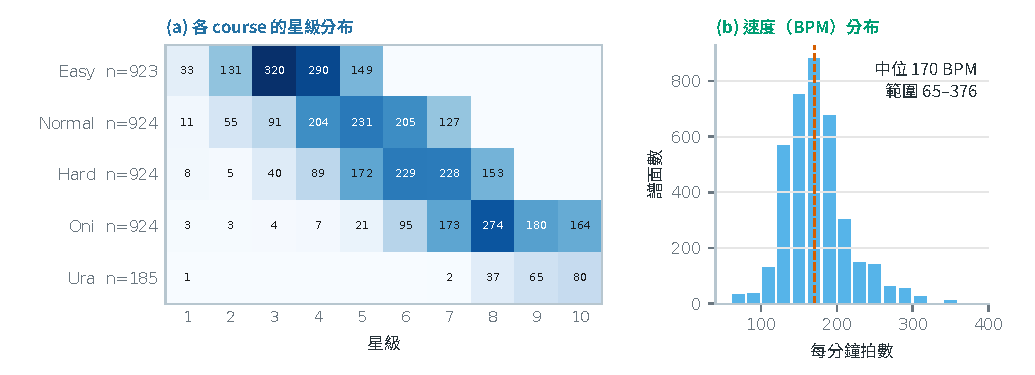
\includegraphics[width=0.98\textwidth]{figs/figCC_corpus_coverage.zh-TW.pdf}
\caption{定義校準範圍的人類參照語料之 course 難度與速度涵蓋。
\textbf{(a)} 3{,}880 張訓練譜中，各 course 的星級計數：每個 course 都橫跨
寬廣且逐步位移的難度範圍。\textbf{(b)} 速度直方圖（中位 170\,BPM，範圍
65--376）。}
\label{fig:coverage}
\end{figure*}

\subsection{資料組建構與完整性}

來源紀錄依 \texttt{group\_id} 與音訊 SHA-256 正規化；不一致的別名會在
資料組索引前排除。測試集依儲存順序包含 120 個歌曲群組，其中第 0--39 組
構成發展組，第 40--119 組構成留出組。在檢視留出結果前，我們先固定資料集
版本、擾動與劑量、目標測量、控制、閾值、校準與分析計畫。

\subsection{複本、完整性與推論單位}

每個非零擾動 cell 與控制條件都使用五個固定的 base seed。複本先在每張譜、
每個劑量內平均。course 只有在原譜值、所有目標
劑量與複本、指定的 sham 及必要控制皆可得時才算完整。歌曲至少有一個完整
course 才進入該檢驗；完整 course 再於歌曲內平均。因此，兩個反應統計量
的推論單位都是歌曲，而非譜面、course 或複本。確定性的 no-op 與缺失 cell
不進入分析。

\subsection{控制檢查與數值不變性}

每項保留測量都進行 identity 重算。音符、作者編定格線與時長共同平移
+1 秒，用於檢查對時間原點的不變性。Don--Ka 音色雙射只用於與音色無關的
時值與密度測量，不作為 grammar 或形式的控制。60\,ms 的 C2 平移則是
只讀譜面密度、grammar 與結構測量的 sham。必要控制未通過時，對應目標
反應便不能視為受到支持。每項測量均採用指定的等價容差與 timestamp
捨入規則。只讀譜面的間隔運算使用整數微秒，比最小報告容差細三個數量級。

\subsection{區間與判定規則}

把輸出定向為越大越好後，第一個統計量是原譜加三個劑量的四種強度，與測量
之間的逐譜 Spearman 相關；四個反應全為常數時，敏感度定義為零。第二個
統計量是定向後的最大劑量值減去指定的 sham。點估計取歌曲層級值的平均。
我們進行 10{,}000 次歌曲群組 bootstrap：次要分析報告 nominal 95\% 區間，
十列主要配對則使用 Bonferroni 校正的 99.5\% 區間。
若至少 72/80 首歌曲可評、所有控制均通過，且兩個調整後上界皆低於零，
該反應即獲支持。調整後下界若為非負，則與預期反應相反；其餘情況視為
無法判定。兩列 C5 輸出必須共同符合規則，但其代數等價性只留下單一有效軸。
C5 LM 使用完整且依儲存順序排列的訓練集、trigram order 3，以及
add-$\alpha=0.05$。

\subsection{樣本數與排除}

留出分析從 333 張譜產生 50{,}283 筆觀察紀錄。C1s 保留 332 個完整
course，C8 保留 330 個，其餘有效配對皆保留 333 個。32 項控制全數通過，
觀察到的最大絕對差異為零。另有 19 個確定性 no-op cell 遭排除。

\FloatBarrier

\section{受控擾動規格}\label{app:corruptions}

\figref{fig:corruptionatlas} 呈現各項擾動所施加的操作性變化，以及預先指定的
目標測量。

\begin{figure*}[t]
\centering
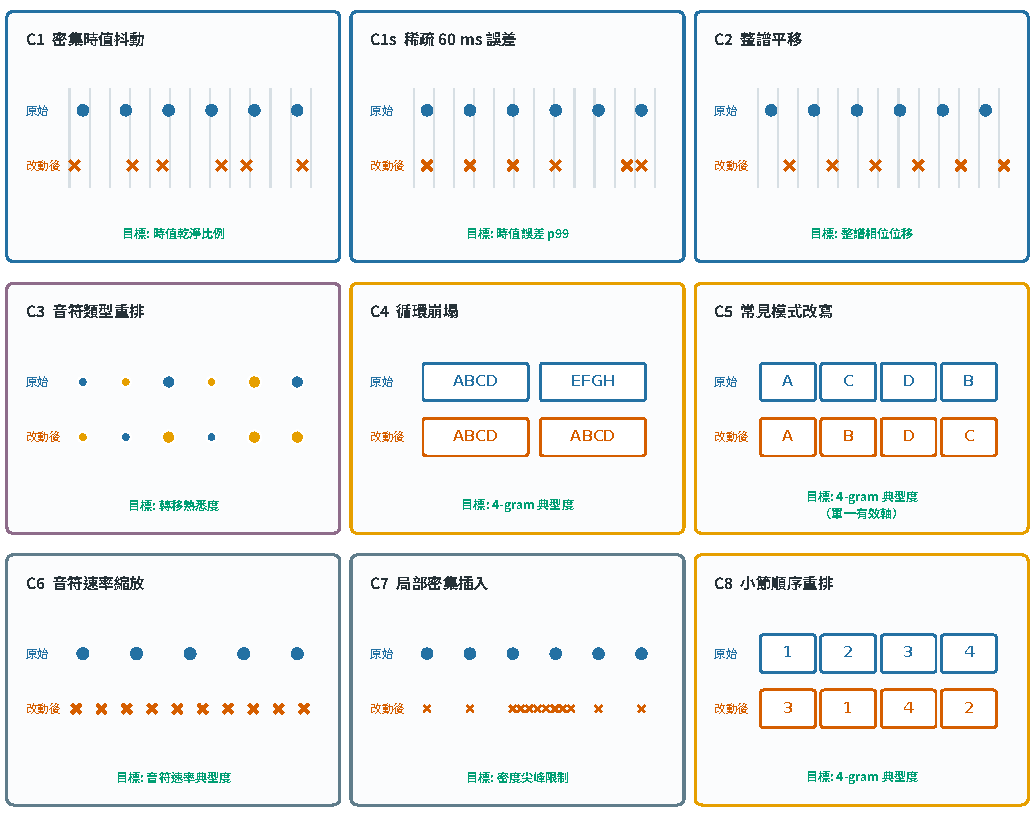
\includegraphics[width=0.975\textwidth]{figs/figP_corruption_atlas.zh-TW.pdf}
\caption{受控擾動圖譜。藍色表示原譜，橘色表示編輯後的事件。各 panel
呈現一種擾動所改變的性質，並標示其目標測量。C1--C2 針對時值，C3 針對
轉移熟悉度，C4--C5 與 C8 針對重複或形式，C6--C7 則針對難度適配與局部
負荷。這些編輯隔離了操作性變化，但不涵蓋譜面品質的所有面向。}
\label{fig:corruptionatlas}
\end{figure*}

170 張譜的發展矩陣在每個非零 cell 使用一個 realization，連同原譜共產生
4{,}760 張變體。C1s 將譜面 $n$ 個音符中的
$\max(1,\operatorname{round}(np))$ 個平移 $\pm60$\,ms。C3--C5 保留音符
時間，C4 與 C6 則保留或控制密度。原始特徵與其衍生分數都在同一批變體上
計算，等價量只計一次。C5 由一個 LM 選擇常見模式改寫，再由另一個獨立擬合
的 LM 評分；perplexity 反轉仍然存在（9.44 $\to$ 6.04，$-36\%$）。

\FloatBarrier

\section{指標指南與延伸結果}\label{app:visuals}

\figref{fig:metricguide} 將各構念連結至所需輸入、代表性輸出與目前最強的
證據；其中的證據標籤區分具留出擾動檢驗的輸出，以及由發展組分析支持的元件。

\begin{figure*}[t]
\centering
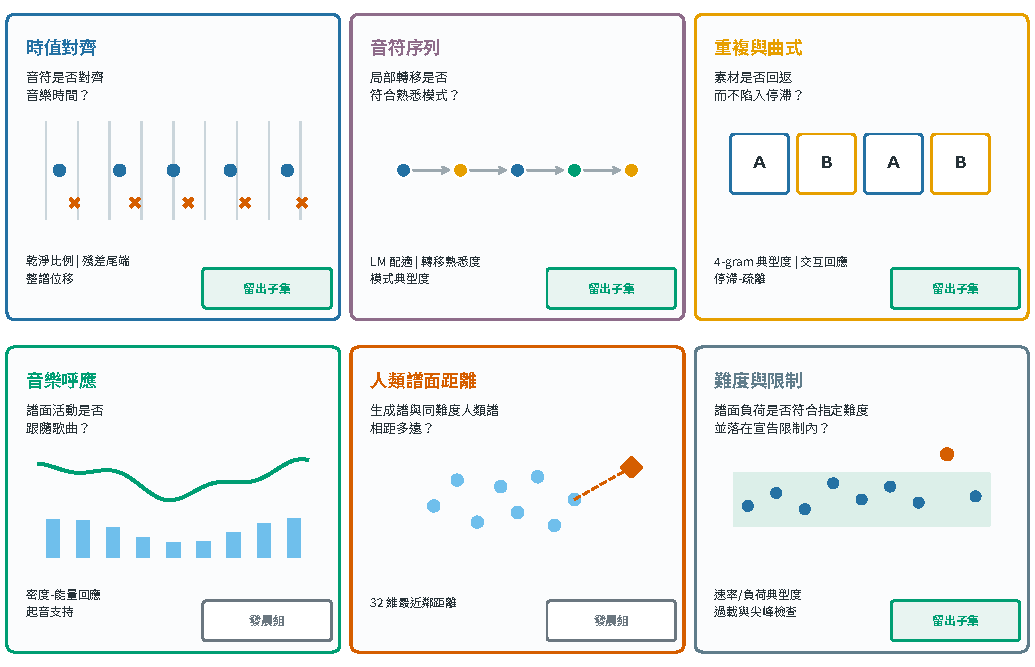
\includegraphics[width=0.98\textwidth]{figs/figM_metric_constructs.zh-TW.pdf}
\caption{指標與構念對照指南。每個 panel 提出一項評估問題，圖示相關訊號，
列出代表性輸出，並標示目前最強的證據。「留出子集」表示只有
\tabref{tab:suite} 中具名的輸出具有留出擾動證據。典型性描述相對同難度
人類範圍的偏離。}
\label{fig:metricguide}
\end{figure*}

\figref{fig:responsemap} 顯示目標擾動可能同時影響多個分數家族，因此這些測量
應以剖面方式解讀，而非視為彼此可交換的孤立讀數。

\begin{figure*}[t]
\centering
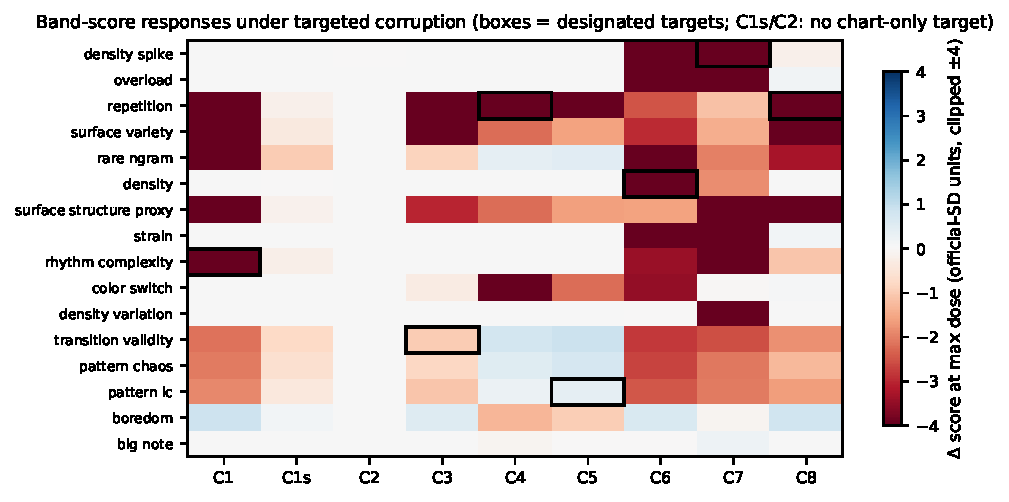
\includegraphics[width=0.94\textwidth]{figs/figC_coupling.pdf}
\caption{14 個非冗餘的校準後只讀譜面分數，對各擾動在發展組最大強度下的
反應。各格涵蓋範圍典型性分數與單側檢查。紅色表示分數下降、藍色表示上升；
數值以人類參照譜的標準差為單位，截斷於 $\pm4$。黑框標示在發展組選出的
目標列，不代表統計顯著性。矩陣同時顯示目標敏感度與跨家族耦合。}
\label{fig:responsemap}
\end{figure*}

\FloatBarrier

\begin{figure*}[t]
\centering
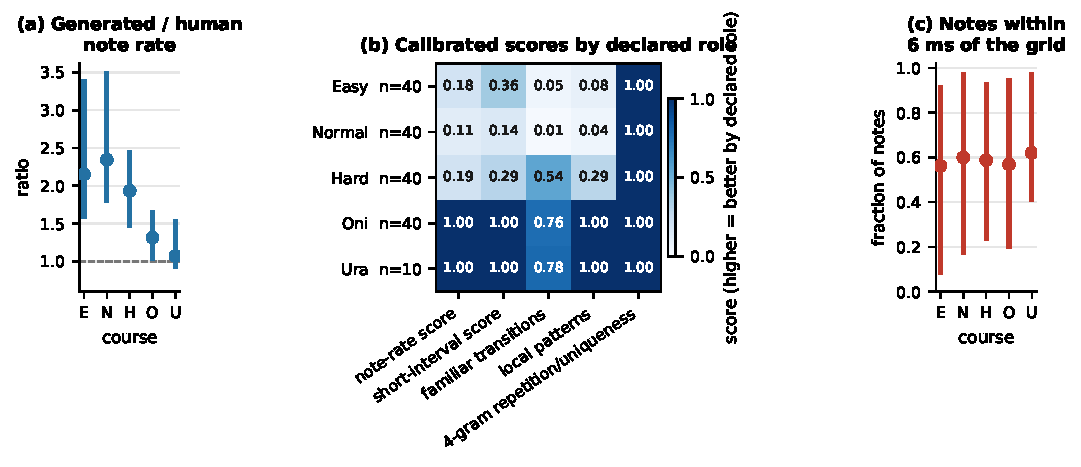
\includegraphics[width=0.96\textwidth]{figs/figE_difficulty.pdf}
\caption{Mapperatorinator 在配對發展譜上的探索性難度剖面。Easy 至 Oni
各含 40 個歌曲--course 配對，Ura 含 10 個。點為中位數，豎線跨第 10 至
90 百分位。生成密度會隨 course 難度提高而接近人類參照，時值卻沒有相同
趨勢；這支持 course 不匹配的解讀，而非高難度下的全面改善。}
\label{fig:difficulty}
\end{figure*}

\FloatBarrier

\section{釋出材料}

程式碼、評估紀錄與繪圖程式公開於 \artifacturl{}。

\bibliographystyle{IEEEtran}
\bibliography{references}

\end{document}
